% generated by romeo (IRCCyN) : a Tool for Time Petri Nets Analysis  

\documentclass[a4paper,10pt]{article}
\usepackage{tikz} 
 \usetikzlibrary{arrows,automata,positioning,petri}

 
\begin{document}
\begin{figure} 
 {\footnotesize 
 \begin{center}
	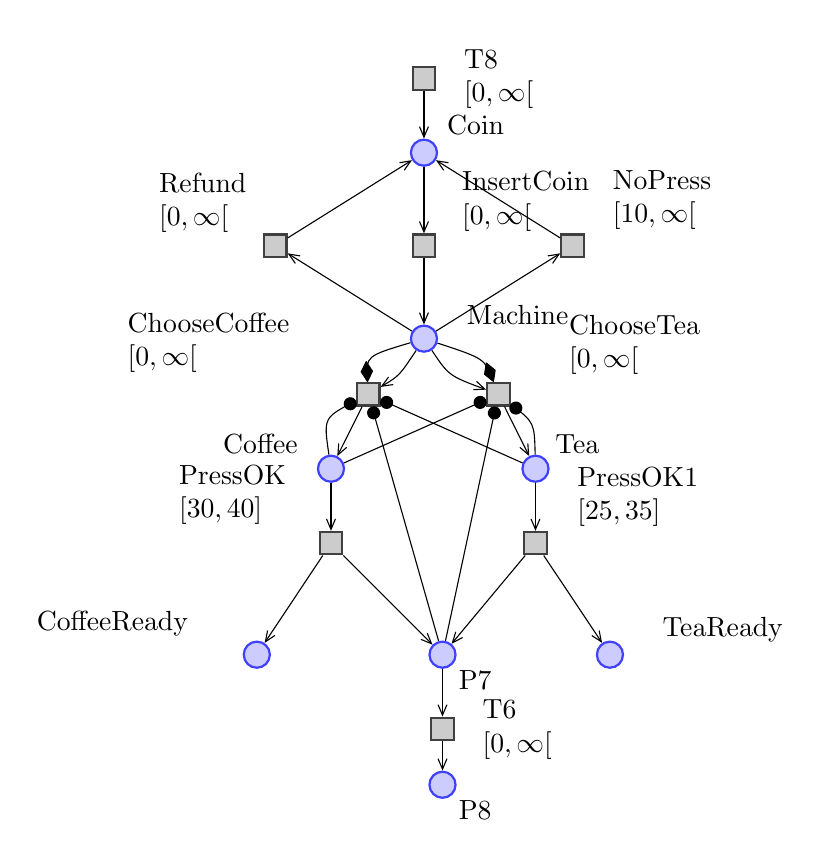
\begin{tikzpicture} 
	 [scale =1] 
	 \tikzset{node distance =0.8955223880597015cm, bend angle=-45,auto}
	\tikzstyle{place}=[circle,thick,draw=blue!75,fill=blue!20,minimum size=9.0 pt]
	\tikzstyle{transition}=[rectangle,thick,draw=black!75,fill=black!20,minimum size=8.1 pt]
	\node [place,tokens=0](p1) at (188.5 pt,-74.3 pt)[label={[label distance=0.7pt]33.1:Coin}]{};
	\node [place,tokens=0](p2) at (188.5 pt,-141.5 pt)[label={[label distance=7.0pt]8.3:Machine}]{};
	\node [place,tokens=0](p3) at (154.9 pt,-188.5 pt)[label={[label distance=3.6pt]166.5:Coffee}]{};
	\node [place,tokens=0](p4) at (228.8 pt,-188.5 pt)[label={[label distance=-1.0pt]27.7:Tea}]{};
	\node [place,tokens=0](p5) at (128.1 pt,-255.7 pt)[label={[label distance=16.5pt]171.8:CoffeeReady}]{};
	\node [place,tokens=0](p6) at (255.7 pt,-255.7 pt)[label={[label distance=10.4pt]4.7:TeaReady}]{};
	\node [place,tokens=0](p7) at (195.2 pt,-255.7 pt)[label={[label distance=-1.8pt]-45.0:P7}]{};
	\node [place,tokens=0](p8) at (195.2 pt,-302.7 pt)[label={[label distance=-1.8pt]-45.0:P8}]{};
	\node [transition] (t1)  at (188.5 pt,-107.9 pt)[label={[label distance=-0.2pt]9.3:\begin{tabular}{l} InsertCoin \\  $ [0,\infty[ $ \end{tabular}}]{};
	\node [transition] (t1)  at (188.5 pt,-107.9 pt)[label={[text=red,label distance=-7.0pt]45.0:\begin{tabular}{l} $  $ \\  \end{tabular}}]{};
	\node [transition] (t1)  at (188.5 pt,-107.9 pt)[label={[text=blue,label distance=-0.7pt]-26.6:\begin{tabular}{l} $  $ \\  \end{tabular}}]{};
	\draw[-angle 45] (p1) edge  (t1) ;
	\draw[-angle 45] (t1) edge  (p2) ;
	\node [transition] (t2)  at (168.4 pt,-161.6 pt)[label={[label distance=14.8pt]170.4:\begin{tabular}{l} ChooseCoffee \\  $ [0,\infty[ $ \end{tabular}}]{};
	\node [transition] (t2)  at (168.4 pt,-161.6 pt)[label={[text=red,label distance=-7.0pt]45.0:\begin{tabular}{l} $  $ \\  \end{tabular}}]{};
	\node [transition] (t2)  at (168.4 pt,-161.6 pt)[label={[text=blue,label distance=-0.7pt]-26.6:\begin{tabular}{l} $  $ \\  \end{tabular}}]{};
	\draw[-angle 45] (p2) .. controls (179.6 pt,-154.9 pt) ..  (t2) ;
	\draw[-diamond] (p2) .. controls (167.5 pt,-147.8 pt) ..  (t2) ;
	\draw[-*] (p3) .. controls (152.2 pt,-170.1 pt) ..  (t2) ;
	\draw[-*] (p4) edge  (t2) ;
	\draw[-*] (p7) edge  (t2) ;
	\draw[-angle 45] (t2) edge  (p3) ;
	\node [transition] (t3)  at (215.4 pt,-161.6 pt)[label={[label distance=11.7pt]9.9:\begin{tabular}{l} ChooseTea \\  $ [0,\infty[ $ \end{tabular}}]{};
	\node [transition] (t3)  at (215.4 pt,-161.6 pt)[label={[text=red,label distance=-7.0pt]45.0:\begin{tabular}{l} $  $ \\  \end{tabular}}]{};
	\node [transition] (t3)  at (215.4 pt,-161.6 pt)[label={[text=blue,label distance=-0.7pt]-26.6:\begin{tabular}{l} $  $ \\  \end{tabular}}]{};
	\draw[-angle 45] (p2) .. controls (197.5 pt,-154.9 pt) ..  (t3) ;
	\draw[-diamond] (p2) .. controls (210.4 pt,-148.7 pt) ..  (t3) ;
	\draw[-*] (p4) .. controls (228.4 pt,-171.9 pt) ..  (t3) ;
	\draw[-*] (p3) edge  (t3) ;
	\draw[-*] (p7) edge  (t3) ;
	\draw[-angle 45] (t3) edge  (p4) ;
	\node [transition] (t4)  at (154.9 pt,-215.4 pt)[label={[label distance=2.4pt]162.4:\begin{tabular}{l} PressOK \\  $ [30,40] $ \end{tabular}}]{};
	\node [transition] (t4)  at (154.9 pt,-215.4 pt)[label={[text=red,label distance=-7.0pt]45.0:\begin{tabular}{l} $  $ \\  \end{tabular}}]{};
	\node [transition] (t4)  at (154.9 pt,-215.4 pt)[label={[text=blue,label distance=-0.7pt]-26.6:\begin{tabular}{l} $  $ \\  \end{tabular}}]{};
	\draw[-angle 45] (p3) edge  (t4) ;
	\draw[-angle 45] (t4) edge  (p5) ;
	\draw[-angle 45] (t4) edge  (p7) ;
	\node [transition] (t5)  at (228.8 pt,-215.4 pt)[label={[label distance=1.2pt]14.9:\begin{tabular}{l} PressOK1 \\  $ [25,35] $ \end{tabular}}]{};
	\node [transition] (t5)  at (228.8 pt,-215.4 pt)[label={[text=red,label distance=-7.0pt]45.0:\begin{tabular}{l} $  $ \\  \end{tabular}}]{};
	\node [transition] (t5)  at (228.8 pt,-215.4 pt)[label={[text=blue,label distance=-0.7pt]-26.6:\begin{tabular}{l} $  $ \\  \end{tabular}}]{};
	\draw[-angle 45] (p4) edge  (t5) ;
	\draw[-angle 45] (t5) edge  (p6) ;
	\draw[-angle 45] (t5) edge  (p7) ;
	\node [transition] (t6)  at (195.2 pt,-282.5 pt)[label={[label distance=0.5pt]0.0:\begin{tabular}{l} T6 \\  $ [0,\infty[ $ \end{tabular}}]{};
	\node [transition] (t6)  at (195.2 pt,-282.5 pt)[label={[text=red,label distance=-7.0pt]45.0:\begin{tabular}{l} $  $ \\  \end{tabular}}]{};
	\node [transition] (t6)  at (195.2 pt,-282.5 pt)[label={[text=blue,label distance=-0.7pt]-26.6:\begin{tabular}{l} $  $ \\  \end{tabular}}]{};
	\draw[-angle 45] (p7) edge  (t6) ;
	\draw[-angle 45] (t6) edge  (p8) ;
	\node [transition] (t8)  at (188.5 pt,-47.5 pt)[label={[label distance=0.5pt]0.0:\begin{tabular}{l} T8 \\  $ [0,\infty[ $ \end{tabular}}]{};
	\node [transition] (t8)  at (188.5 pt,-47.5 pt)[label={[text=red,label distance=-7.0pt]45.0:\begin{tabular}{l} $  $ \\  \end{tabular}}]{};
	\node [transition] (t8)  at (188.5 pt,-47.5 pt)[label={[text=blue,label distance=-0.7pt]-26.6:\begin{tabular}{l} $  $ \\  \end{tabular}}]{};
	\draw[-angle 45] (t8) edge  (p1) ;
	\node [transition] (t11)  at (134.8 pt,-107.9 pt)[label={[label distance=-3.6pt]167.2:\begin{tabular}{l} Refund \\  $ [0,\infty[ $ \end{tabular}}]{};
	\node [transition] (t11)  at (134.8 pt,-107.9 pt)[label={[text=red,label distance=-7.0pt]45.0:\begin{tabular}{l} $  $ \\  \end{tabular}}]{};
	\node [transition] (t11)  at (134.8 pt,-107.9 pt)[label={[text=blue,label distance=-0.7pt]-26.6:\begin{tabular}{l} $  $ \\  \end{tabular}}]{};
	\draw[-angle 45] (p2) edge  (t11) ;
	\draw[-angle 45] (t11) edge  (p1) ;
	\node [transition] (t12)  at (242.2 pt,-107.9 pt)[label={[label distance=0.6pt]14.0:\begin{tabular}{l} NoPress \\  $ [10,\infty[ $ \end{tabular}}]{};
	\node [transition] (t12)  at (242.2 pt,-107.9 pt)[label={[text=red,label distance=-7.0pt]45.0:\begin{tabular}{l} $  $ \\  \end{tabular}}]{};
	\node [transition] (t12)  at (242.2 pt,-107.9 pt)[label={[text=blue,label distance=-0.7pt]-26.6:\begin{tabular}{l} $  $ \\  \end{tabular}}]{};
	\draw[-angle 45] (p2) edge  (t12) ;
	\draw[-angle 45] (t12) edge  (p1) ;
	\end{tikzpicture} 
 \end{center} 
 } 

 \end{figure}

 
\end{document}
